\startcontents[localtoc]
\printcontents[localtoc]{}{0}{\subsection*{Contents}\setcounter{tocdepth}{2}}



\phantomsection
\addcontentsline{toc}{section}{Set example data}
\subsubsection*{Set example data}



Set independent and dependent variables for \texttt{wlsfit} algorithm, OLS method.
Lets operate in semi logarithm space for easy plotting.

\begin{lstlisting}
DIols = [];
DIols.x.v = log10([10 1e2 1e3 1e4 1e5]);
DIols.x.u = [];
DIols.y.v = [19.700 32.700 69.700 90.700 148.700];
% polynomial order:
DIols.n.v = 2;

% Create data for WLS method (add uncertainties of y):
DIwls = DIols;
DIwls.y.u = [4 10 13 20 33];
\end{lstlisting}


\phantomsection
\addcontentsline{toc}{section}{Call algorithm}
\subsubsection*{Call algorithm}



Use QWTB to apply algorithm \texttt{wlsfit} to data \texttt{DIwls}.

\begin{lstlisting}
DOols = qwtb('wlsfit', DIols);
DOwls = qwtb('wlsfit', DIwls);
\end{lstlisting}
\begin{lstlisting}[language={},xleftmargin=5pt,frame=none]
QWTB: no uncertainty calculation
QWTB: wlsfit wrapper: No y uncertainties nor weights -> using OLS fitting
QWTB: no uncertainty calculation
QWTB: wlsfit wrapper: Using WLS fitting based on y uncertainties.

\end{lstlisting}


\phantomsection
\addcontentsline{toc}{section}{Display results}
\subsubsection*{Display results}



Results is

\begin{lstlisting}
disp('')
disp([DOols.model.v ':'])
disp(['offset          : ' num2str(DOols.coefs.v(1)) ' +- ' num2str(DOols.coefs.u(1))])
disp(['linear coeff.   : ' num2str(DOols.coefs.v(2)) ' +- ' num2str(DOols.coefs.u(2))])
disp(['quadratic coeff.: ' num2str(DOols.coefs.v(3)) ' +- ' num2str(DOols.coefs.u(3))])
disp([DOwls.model.v ':'])
disp(['offset          : ' num2str(DOwls.coefs.v(1)) ' +- ' num2str(DOwls.coefs.u(1))])
disp(['linear coeff.   : ' num2str(DOwls.coefs.v(2)) ' +- ' num2str(DOwls.coefs.u(2))])
disp(['quadratic coeff.: ' num2str(DOwls.coefs.v(3)) ' +- ' num2str(DOwls.coefs.u(3))])
\end{lstlisting}
\begin{lstlisting}[language={},xleftmargin=5pt,frame=none]

Ordinary Least Squares:
offset          : 14.5 +- 2.1448
linear coeff.   : -0.11429 +- 1.6345
quadratic coeff.: 5.2857 +- 0.26726
Weighted Least Squares, weights based on u(y):
offset          : 12.6828 +- 16.9884
linear coeff.   : 1.9434 +- 19.1198
quadratic coeff.: 4.9055 +- 3.9754

\end{lstlisting}


\phantomsection
\addcontentsline{toc}{section}{Interpolate values}
\subsubsection*{Interpolate values}



Interpolate fitted polynom at values \texttt{t}.

\begin{lstlisting}
t = [0:0.1:6];
tyols = DOols.func.v(t, DOols.coefs.v);
tywls = DOwls.func.v(t, DOwls.coefs.v);
\end{lstlisting}


Calculate uncertainties of interpolated values (\texttt{S} is sensitivity matrix, \texttt{CC} is covariance
matrix of coefficients, \texttt{CT} is covariance matrix of interpolated values, \texttt{uty} is uncertainty of
interpolated values).

\begin{lstlisting}
for i = 1:length(t);
        S = t(i).^[0:DIols.n.v];
        CC = diag(DOols.coefs.u,0)*DOols.coefs.c*diag(DOols.coefs.u,0);
        CT(i)=S*CC*S';
end
utyols=CT.^0.5;

for i = 1:length(t);
        S = t(i).^[0:DIwls.n.v];
        CC = diag(DOwls.coefs.u,0)*DOwls.coefs.c*diag(DOwls.coefs.u,0);
        CT(i)=S*CC*S';
end
utywls=CT.^0.5;
\end{lstlisting}


\phantomsection
\addcontentsline{toc}{section}{Plot results}
\subsubsection*{Plot results}

\begin{lstlisting}
hold on
% input data:
errorbar(DIwls.x.v, DIwls.y.v, DIwls.y.u, 'xb')
% outputs:
plot(DIols.x.v, DOols.yhat.v, 'or')
errorbar(DIwls.x.v, DOwls.yhat.v, DOwls.yhat.u, 'og')
plot(t, tyols, '--r');
plot(t, tywls, '-g');
plot(t, tyols + utyols, '--r');
plot(t, tywls + utywls, '-g');
plot(t, tyols - utyols, '--r');
plot(t, tywls - utywls, '-g');
xlabel('log(f)')
ylabel('error of amplitude')
legend('original data','fitted values, OLS', 'fitted values, WLS','interpolated values, OLS', 'interpolated values, WLS', 'uncer. of int. val., OLS', 'uncert. of int. val., WLS','location','southeast')
hold off
\end{lstlisting}
\begin{center}
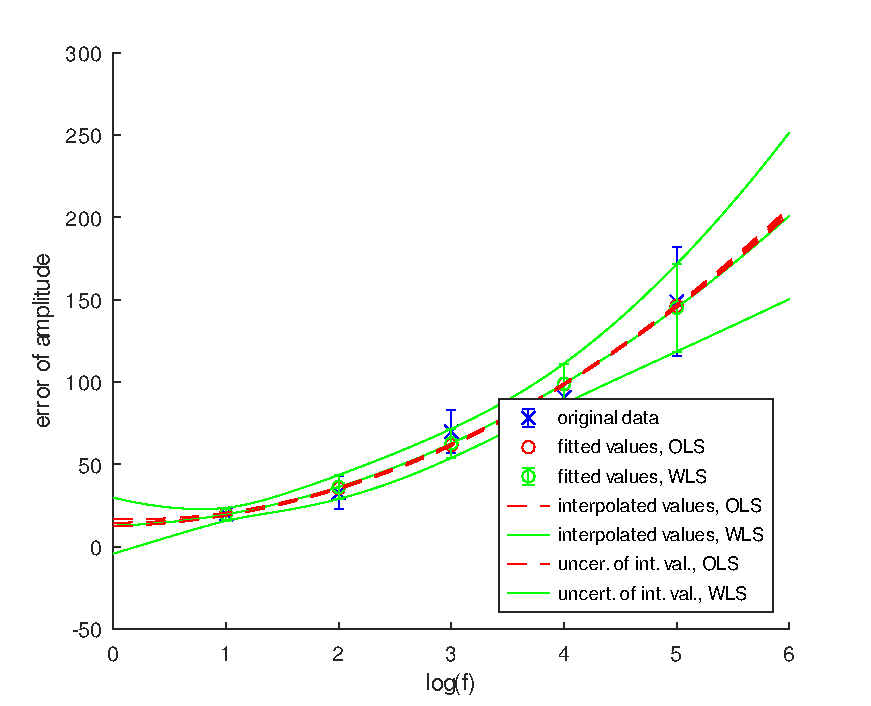
\includegraphics[width=0.7\textwidth]{algs_examples_published/wlsfit_alg_example-1.pdf}
\end{center}


\stopcontents[localtoc]
